\section{Case study}
\label{sec:case_study}

\begin{table*}[t]
    \centering
    \begin{tabular}{c c c c c c}
    \hline
        Case & Categories & Controllers & Properties & Behaviors  \\ 
        \hline
        D1(R) & Conflicted config & Deployment + Kubelet & Liveness & Scheduling and evicting pods infinitely  \\ 
        H1(R) & Lack of context & HPA + App CPU changes & Safety & HPA is agnostic to app  \\ 
        H2(R) & Conflicted config & HPA + Deployment & Safety & Sub-optimal scaling behavior  \\ 
        H3(R) & Imperfect knowledge & HPA + Node reachability & Safety & Semantically wrong avg CPU util (reachability vs healthiness)  \\ 
        S1 & Conflicted config & Scheduler + Descheduler & Liveness & High utilization(scheduler) <-> Low utilization(descheduler) \\ 
        S2(R) & Conflicted config & Scheduler + Descheduler & Liveness & Deployment preference <-> Violation in maxSkew \\ 
        S3(R) & Conflicted config & Scheduler & Liveness & Two pod spread constraints are conflicted each other  \\ 
        S5 & Conflicted config & Scheduler & Safety & Pods are scheduled to one node, because of lopsided preference  \\ 
        S6(R) & Lack of feature & Scheduler & Safety & Scheduler is not able to adjust skewed placement  \\ 
        S7(R) & Lack of context & Scheduler + Kubelet & Liveness & Scheduler includes NotReady node for maxSkew calculation  \\ 
        \hline
    \end{tabular}
    \caption{Summary of multi-controller failure cases. Reproduced cases are marked with (R).}
    \label{table:summary}
\end{table*}

\subsection*{Failure cases}
In this section, we will walk through 10 failure cases to provide overall picture of how multi-controller can fall apart. All failure cases are elephant in the room. Clearly the problem exists right there in the cluster, nibbling away at cluster resources but none of controllers can recognize it or fix it.  \textit{S3} case will not be described in this paper. It is explained in Kubernetes official document ~\cite{}.

\paragraph*{D1, Deployment + Kubelet}
Deployment controller has \textit{nodename} configuration which is one way of restricting pods from the deployment to run in a specific node. In this example, deployment specifies \textit{node-1} for scheduling pods.
On the other hand, a node can be marked by taint configuration to restrict pods that can be scheduled in this node. Pod having corresponding \textit{Toleration} only is allowed be scheduled or run in the tainted node. \textit{NoExecute} taint will not let non-tolerated pods scheduled and already running non-tolerated pods will be all evicted from the node.
\textit{nodename} and \textit{NoExecute taint} tries to do exactly the opposite scheduling. It will create infinite loop of Deployment controller scheduling pods to node-1 and Kubelet controller evicting pods from node-1. Apparently it is not prohibited to form a vicious scheduling cycle. Furthermore, \textit{TerminationGracePeriodSeconds} configuration in deployment lets you handle termination gracefully (default: 30s). Pods will stay in \textit{terminating} status for \textit{TerminationGracePeriodSeconds} before being terminated completely. It can result in a large number of pods in \textit{terminating} status, still taking up cluster resources. 

\paragraph*{H1, HPA + App CPU utilization change}
\textit{Horizontal Pod Autoscaler (HPA)} is in charge of automatically scaling up and down based on defined scaling rule (default: 50\% CPU utilization). If average pod CPU utilization of a deployment exceeds 50\%, HPA will create new pods to satisfy the target metric value. 
% \begin{equation}
% desiredReplicas = ceil[currentReplicas * ( currentMetricValue / desiredMetricValue )]
% \end{equation}
HPA does not take into consideration why CPU utilization increases. One common source of increase in CPU utilization could be surge in the number of incoming requests. In this case, scaling up is valid reaction. However, there are other sources of CPU usage. For example, garbage collection, initilization phase of application or any other forms of computation happening inside application are going to increase CPU utilization as well. For these cases, even if scaling up will not help to reduce the CPU utilization, it will scale up since HPA differentiate where CPU increase comes from. Unintended scale up is critical issue, leading to increase in cost. Again, note that none of application and HPA controller is doing anything wrong individually.

\paragraph*{H2, Deployment + HPA}
You can specify the number of replicas in deployment configuration (Default: 1). A deployment is applied with empty replica field and it creates 1 replica. HPA is applied later with configuration of 6 minimum replica and now the number of replicas becomes 6. At some point, you applied a new configuration for the deployment and at this time, the replica field is defined to 3. One of two controllers' replica configuration should be ignored. However, what happens is the number of replicas becomes 3 temporarily for a few seconds by deployment and 6 again by HPA. If the intented number of replica is 6, the change is sub-optimal. If the intent is 3, it fails due to duplicate configuration.

\paragraph*{H3}

\paragraph*{S1, Scheduler + Descheduler}
Scheduler and Descheduler could be configured to prefer low utiliation node or high utilization node. Default behavior of scheduler is spreading pods as much as it can to make it more fault-tolerant. The purpose of preferring high utilization node is to enable bin packing, retains less number of nodes required to run the cluster and save the overall cost. Unnecessary scheduling and descheduling cycle could be created by confliction between the two controllers. Scheduler is configured to place pods in high utilization node and descheduler is condfigured to evict pods from high utilization node. 

\paragraph*{S2, Daemonset + Descheduler}
\textit{Daemonset} will manage a part of scheduling rule. One of them is \textit{NodeAffinity}. It schedules pods based on affinity weight. The problematic situation is daemonset checks the node affinity and scheduler keeps placing pods in node-1. At the same time, descheduler is running with \textit{RemoveDuplicate} configuration which forces only one pod to run in a node and evicts the rest of them. It is per deployment policy. NodeAffinity and RemoveDuplicate are conflicted each other and will create endless cycle of termination, eviction and creation of pod. 
\textit{S5} arises in a similar fashion by image locality config in deployment and descheduler.

\paragraph*{S6, Node maintenance + Scheduler}
From time to time, nodes could be put in maintenance, for example to add a new library, update security feature. Onec the node is shut down, pods in the node will be terminated and scheduled to another node. For instance, there are three nodes and three replica, one replica running in each node. The node-1 is going through the maintenance and automatically the pod running there is moved to the node-2. The overall placement becomes skewed but it is the best possible movement at the moment. Later, the maintenance finishes and node-1 begins operation again. The expectation is rebalancing the pod spread by moving one pod from node-2 to node-1. Apparently, it will not happen unless descheduler is installed with right plugin (Descheduler is not default controller). This is not the optimal placement and reduces availability by failing appropriate pod spread. 


\paragraph*{S7, Scheduler + Kubelet}
In this failure case, scheduler is configured with maxSkew of 1. Maximum skewness allowed is 1. The deployment creates 3 pods and scheduler will place one pod per a node, pod-\textit{\{1,2,3\}} in node-\textit{\{1,2,3\}} respectively in this example. However, node-3 becomes \textit{NotReady} since kubelet in node-3 is unreponsive for some reason. Pod-3 is not able to be scheduled or will be evicted if it was running. It is expected that node-3 should not be counted when censoring the maxSkew and pod-3 is still scheduled in one node among healty nodes, node-1 and node-2. It does not violate maxSkew:1 rule (two pods in node-1 and one pod in node-2 or the other way around). What actually happens is pod-3 will not be scheduled and remains pending indefinitely since node-3 is still included for maxSkew calculation. It needs to be investigaed further to diagnose the root cause. Regardless of why it occurs, it is counter-intuitive to human that a pod cannot be scheduled due to unresponsive node. It means it is hard to diagnose it when it happens and Kuberentes again does not alert any warning. It is another potential black hole that will suck human resources, wasting their time to look into the issue.


\subsection*{How are these failures created at the first place?}
Large systems are developed by people in different teams and different organizations. One team or a certain group of people in case of open source is responsble for developing and maintaining a certain part out of the entire system. It is impossible for them to know how all other parts of the system function in detail. It is not feasible to write a controller not incuring any conflicted cases with all other controller for all possible cases. Even if it is technically possible, it is not even desirable because then the development process will take exhastively long time.
The programming model of the large system including Kubernetes is another contributer to this type of failure. We will use Kubernetes to describe more detailed example. What each controller does in Kubernetes is periodically monitoring if the associated part in the cluster is currently in desirable status or not. If it is not, it will try to bring it back to the desirable status, running built-in logic of the controller. For example, Horizontal Pod Autoscaler(HPA) scales up the number of pods if CPU utilization becomes higher than 50\% (it is configurable). This specific model is called reconciliation. During reconciliation The important part is a controller does not take into account what other controllers are doing and how they can react to its action. It simply sees the current status of the cluster and run its own logic to put the cluster back to the right place.
Even within one controller, there could be multiple configurations which are functionally not exclusive each other. For exapmle, Deployment could be configured with multiple \textit{Pod Topology Spread Constraint} policies and currently Kubernetes does not have safety net guaranteeing that the configurations are not contradictorial or any kind of alerting system warning it is contradictorial. It is completely at your own risk.


\subsection*{Why is it hard to prevent these failures?}
If it is evident that the system could fall into already known precarious status when the cluster is deployed with self-destroying configuration, why were they not fixed already? It is not because it is such a huge system and the community is large enough or active to resolve these problems. It is because they are not trivial problems. Note that each part of the system is not doing anything wrong if you look at them individually and there is no bug in the code.
It is inherently ambiguous to classify such failure cases as bug. Each controller is working as it is supposed to do and clearly there is no bug in its logic if you look them individually. Some of answers against reported github issues was that developers in Kubernetes community maintaining the controller are aware of or admit that is the issue but they ended up not fixing or not being able to fix it while saying it is their design choice or there is no clear way to patch it. The clear solution does not exist since multiple parties in the system are involved and tangled each other. It is not because Kubernetes community constantly procrastinates or neglects them. 
Most of these problems we are presenting in this paper could be prevented if you know it will happen before you apply them to your cluster. For the example in D1 failure case, if you had known that Deployment configuration and Scheduler policy are contradictorial each other, you would have not configured in such self-destroying way. However, there are several reasons that it is still not trivial to avoid this type of failures. The first reason is scalability. The nubmer of pods could be easily over a thousand and the number of services deployed in the cluster could be easily over a hundred. To configure this scale of Kubernetes cluster having different applications running, you may need to manage a large number of configuration yaml files for each deployment, nodes, hpa, schedulers, etc. In this scale and complexity, it is challenging to make all controllers always in a coordinated manner in the cluster-wise level. The second reason is that in a large scale cluster some failrues are not noticeable and slowly gnawing the cluster's resources. For example, in S1 failure case, node utilization on average could stay within some range in the half way of scheduler config and deschduler config. It is possible that the cluster resource utilization looks stable even though what is happening beind is deschduler keeping evicting pods from high utilization node and scheduler placing pods in low utilization node makig the utilization high again. The third reasons is that semantically contradictorial configurations does not mean it will always lead to failrues. Many of these problems are triggered in a specific number of nodes and pods. 

\subsection*{Common patterns in multi-controller failure cases}
Table.1 summarizes the failure cases we analyzed and reproduced in this paper. 10 failure cases are analyzed and 8 out of 10 are reproduced in Kubernetes cluster. KinD cluster was used for failure reproduction.

\paragraph*{Scheduling behavior is involved in most of failure cases} 7 out 10 failure cases are directly or indirectly associated with scheduler. Some failure cases does not even require multiple controllers, e.g., S3, S5, S7. Even two conflicted configurations within a scheduler controller can result in failure. Kubernetes is composed of numerous controllers and other system components. Notably the schduler is one of the most complicated controllers. In addition how complicated it is, there are two fundamental design choices of kube-scheduler causing these failures. First, kube-scheduler does not revisit its previous scheduling decision. Once it schedules a pod in a node, the pod will never be re-scheduled to another node unless it is forced by external events like node failure or node taint. Kube-scheduler tries best effort at the time of scheduling and hands off. Even if first placement met all scheduling requirements, it can be violated later by future events. In S6 case, when pods were scheduled, they were spread by default scheduler policy. However, placement becomes skewed when the third node goes into maintenance and all pods in the node are evicted and scheduled in other nodes. Even after the third node becomes alive and able to host pods, the scheduler will not fix the skewed placement. 

\paragraph*{Needs middle layer tools}
As confirmed in the failure case study, Kubernetes currently does not have any type of system layer preventing or warning configurations violating safety or liveness property. It is intrinsically challenging for Kubernetes to support additionaly prevention layer of safety and liveness property. There are three reasons that positions it in fundamentally difficult problem. 
First, there is no way to express user's intent in the current Kubernetes version. Someone might say just implementing a new layer doing that particular job will solve the problem. However, it is not trivial in which way users should express their intents. Which format should new commands look like, which commands should be added, etc. On top of that, it is putting extra burden to users who needs to learn additional commands. Kubernetes configurations are already sufficiently complicated. 
Second, to avoid multi-controller problems at the first place, one possible rather blind solution is removing features that contributes to potentially contradictorial configurations existing in mutliple controllers. For example, MostAllocated config in scheduler and high node utilization plugin in descheduler are pursuing the opposite purpose. One is trying to do bin packing (placing pods in high utilization node) and the other is trying to evict pods from high utilization nodes, hoping them to be scheduled in low utilization node. We can circumvent this probable multi-controller confliction by deprecating high node utilization plugin in descheduler. The same goal can be fulfilled by appropriate pod spreading configuration in scheduler. Although they might represent the same goal in high level, it can never be exactly same. It is simply because the mechanisms they achieve it are different - one is schedule and the other is eviction. They are in charge of exclusive roles.
Third, the confliction does not manifest always by turning on those plugins. It also depends on the exact configurations like threshold for each setting. Deleting conflicted features is overkill since the presence of potential confliction does not always lead to problem as well as it is not appropriate solution since their functionalities are fundamentally different.
Our conclusion is a need for middle layer verification tool. It takes input of Kubernetes yaml config files as they are and outputs whether that certain combination of configurations contains potential multi-controller problems. This new middle layer tool cannot fix the problem automatically since it still is not able to figure out user's intent and it should not be designed to do that because it would be too complicated. The new layer execution should happen offline or at least should be run in background. In other words, ti should not be in the critical path that can hurt the performance of cluster management task. We do not know what the most suitable verification technique is for this problem. We leave it for future work.


\paragraph*{Reproduced in a small scale} The first common pattern is all of failure cases presented in this paper does not need large scale cluster to reproduce them. Maximum number of nodes and pods used for reproduction are 3 and 6 respectively. It implies that they are substances of large scale cluster. When building testing tool or verification program, this observation can be leveraged to help their algorithms to be more efficient by reducing search space it needs to explore.



\begin{figure}[h]
    \centering
    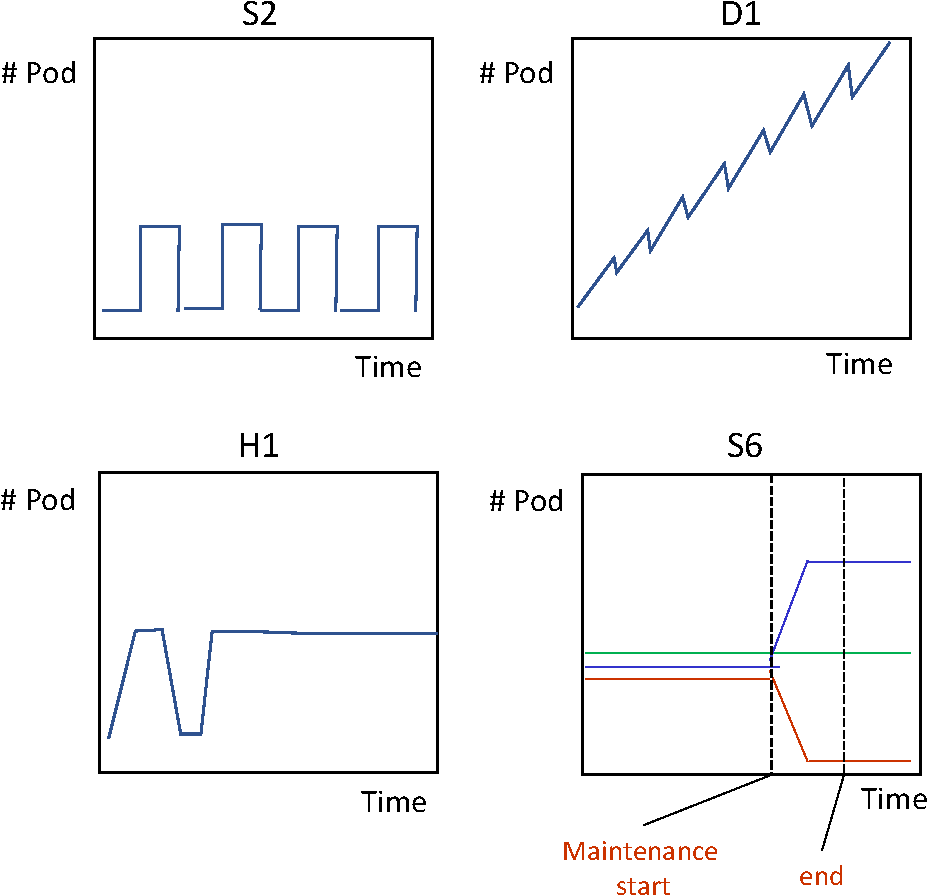
\includegraphics[width=0.4\textwidth]{figure/num_pod.pdf}
    \caption{Number of pods over time for four failure cases.}
    \label{fig:num_pod}
\end{figure}